\section{Rancangan Solusi}

Dibangun sebuah rancangan solusi berupa skenario pengujian yang dilakukan dalam penelitian tugas akhir, yang dapat dilihat pada Gambar \ref{fig:rancangan-solusi}. Berdasarkan Gambar \ref{fig:rancangan-solusi}, tidak ditambahkan dataset baru, melainkan menggunakan dataset yang sudah disediakan pada IndoLEM. Teknik PEFT yang digunakan adalah LoRA (\textit{Low-Rank Adaptation}), \textit{Prefix-Tuning}, dan \textit{Bottleneck Adapter}. Hasil pengujian berupa kinerja dari teknik PEFT serta penggunaan sumber daya dari setiap eksperimen.

\begin{figure}[ht]
    \centering
    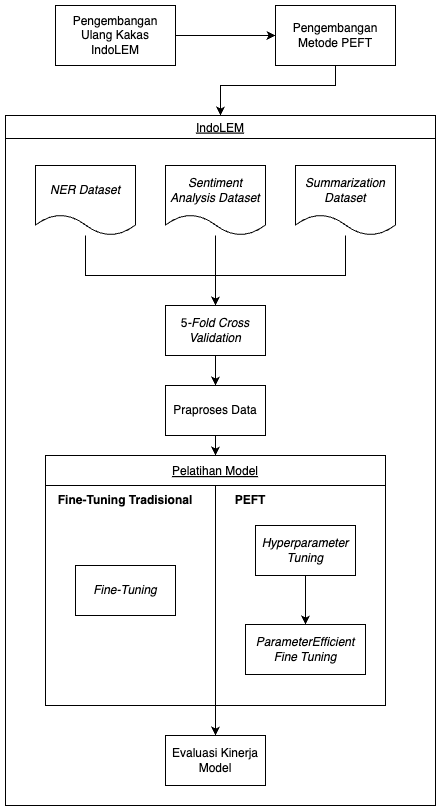
\includegraphics[width=1\textwidth]{chapter-3/rancangan_solusi.png}
    \caption{Rancangan Solusi}
    \label{fig:rancangan-solusi}
\end{figure}
